\section{Undetermined Coefficients [25\%]}
States $u_i$ are given at three nodes in a non-uniform, one-dimensional grid, as shown below.  Using the method of undetermined coefficients, derive the most accurate formula for $du/dx$ at node 2, and give the order of accuracy, with respect to $h$, of your formula.


\begin{figure}[h]
    \centering
    

\tikzset{every picture/.style={line width=0.75pt}} %set default line width to 0.75pt        

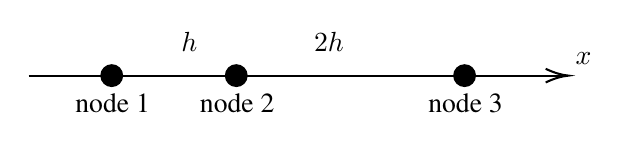
\begin{tikzpicture}[x=0.75pt,y=0.75pt,yscale=-1,xscale=1]
%uncomment if require: \path (0,300); %set diagram left start at 0, and has height of 300

%Straight Lines [id:da5299394466860707] 
\draw    (155,65) -- (413,65) ;
\draw [shift={(415,65)}, rotate = 180] [color={rgb, 255:red, 0; green, 0; blue, 0 }  ][line width=0.75]    (10.93,-3.29) .. controls (6.95,-1.4) and (3.31,-0.3) .. (0,0) .. controls (3.31,0.3) and (6.95,1.4) .. (10.93,3.29)   ;
%Shape: Circle [id:dp0275755717354893] 
\draw  [fill={rgb, 255:red, 0; green, 0; blue, 0 }  ,fill opacity=1 ] (190,65) .. controls (190,62.24) and (192.24,60) .. (195,60) .. controls (197.76,60) and (200,62.24) .. (200,65) .. controls (200,67.76) and (197.76,70) .. (195,70) .. controls (192.24,70) and (190,67.76) .. (190,65) -- cycle ;
%Shape: Circle [id:dp16091151773278578] 
\draw  [fill={rgb, 255:red, 0; green, 0; blue, 0 }  ,fill opacity=1 ] (250,65) .. controls (250,62.24) and (252.24,60) .. (255,60) .. controls (257.76,60) and (260,62.24) .. (260,65) .. controls (260,67.76) and (257.76,70) .. (255,70) .. controls (252.24,70) and (250,67.76) .. (250,65) -- cycle ;
%Shape: Circle [id:dp2533213412832751] 
\draw  [fill={rgb, 255:red, 0; green, 0; blue, 0 }  ,fill opacity=1 ] (360,65) .. controls (360,62.24) and (362.24,60) .. (365,60) .. controls (367.76,60) and (370,62.24) .. (370,65) .. controls (370,67.76) and (367.76,70) .. (365,70) .. controls (362.24,70) and (360,67.76) .. (360,65) -- cycle ;

% Text Node
\draw (227,42.4) node [anchor=north west][inner sep=0.75pt]    {$h$};
% Text Node
\draw (291,42.4) node [anchor=north west][inner sep=0.75pt]    {$2h$};
% Text Node
\draw (176,72) node [anchor=north west][inner sep=0.75pt]   [align=left] {{\fontfamily{ptm}\selectfont node 1}};
% Text Node
\draw (236,72) node [anchor=north west][inner sep=0.75pt]   [align=left] {{\fontfamily{ptm}\selectfont node 2}};
% Text Node
\draw (346,72) node [anchor=north west][inner sep=0.75pt]   [align=left] {{\fontfamily{ptm}\selectfont node 3}};
% Text Node
\draw (417,52.4) node [anchor=north west][inner sep=0.75pt]    {$x$};


\end{tikzpicture}

    \caption{Undetermined coefficients non-uniform, one-dimensional grid.}
\end{figure}


\vspace{-0.5in}
\begin{align*}
    \shortintertext{First I will consider forward, backward, and central differences\newline \textbf{\underline{Forward Difference:}}}
    \sum_{i=2}^{3}\ a_i u_i & = a_2u_2 + a_3u_3\\
    u_3 & \approx u_2 + 2hu' + \frac{1}{2}(2h)^2u'' + \frac{1}{6}(2h)^3u'''\\
    \frac{du}{dx}|_{2} & = a_2u_2 + a_3 \left( u_2 + 2hu' + \frac{1}{2}(2h)^2u'' + \frac{1}{6}(2h)^3u'''\right)\\
    \shortintertext{This gives the following systems of equations,}
    a_2 + a_3 & = 0,\quad 2ha_3  = 1\ \text{Solving gives,}\ a_3 = \frac{1}{2h}, \quad a_2 = -\frac{1}{2h}\\
    \frac{du}{dx}|_{2} & \approx \frac{1}{2h}(u_3 - u_2)\\
    a_3 2h^2u'' & \rightarrow \frac{1}{2h}2h^2u'' \rightarrow hu'',\quad \mathcal{O}(h) \rightarrow \text{First-Order}\\
    \shortintertext{\textbf{\underline{Backward Difference:}}}
    \sum_{i=1}^{2}\ a_i u_i & = a_1u_1 + a_2u_2\\
    u_1 & \approx u_2 + (-h)u' + \frac{1}{2}(-h)^2u'' + \frac{1}{6}(-h)^3u'''\\
    \frac{du}{dx}|_{2} & = a_1(u_2 + (-h)u' + \frac{1}{2}(-h)^2u'' + \frac{1}{6}(-h)^3u''') + a_2u_2\\
    a_1 + a_2 & = 0, \quad -ha_1  = 1,\ \text{Solving gives,}\ a_1 = -\frac{1}{h}, \quad a_2 = \frac{1}{h}\\
    \frac{du}{dx}|_{2} & \approx \frac{1}{h}(u_2 - u_1)\\
    a_1\frac{h^2}{2}u'' & \rightarrow -\frac{1}{h}\frac{h^2}{2}u'' \rightarrow -\frac{h}{2}u'', \quad \mathcal{O}(h) \rightarrow \text{First-Order}
\end{align*}


\pagebreak
\pagestyle{fancy}
\restoregeometry


\vspace{-0.5in}
\begin{align*}
    \shortintertext{\textbf{\underline{Central Difference:}}}
    \sum_{i=1}^3 & = a_1 u_1 + a_2u_2 + a_3u_3\\
    \shortintertext{Using the expressions for $u_1$ and $u_3$ from forward and backward gives,}
    & a_1(u_2 - hu' + \frac{1}{2}h^2u'' - \frac{1}{6}h^3u''')+\ldots\\
    & a_2u_2+\ldots\\
    & a_3(u_2+2hu' + 2h^2u'' + \frac{4}{3}h^3u''')\\
    \shortintertext{This gives the following systems of equations,}
    & a_1 + a_2 + a_3 = 0\\
    & -ha_1 + 2ha_3 = 1\\
    & \frac{1}{2}h^2a_1 + 2h^2a_3 = 0\\
\end{align*}

\vspace{-0.75in}
\begin{align*}
    \shortintertext{Solving for $a_1,\ a_2,\ a_3$ gives,}
    a_1 = -\frac{2}{3h},\quad & a_2 = \frac{1}{2h}, \quad a_3 = \frac{1}{6h}
    \shortintertext{This gives that the approximation is,}
    \frac{du}{dx}|_2 & \approx \frac{1}{6h}\left(u_3 + 3u_2 - 4u_2\right)\\
    \shortintertext{Finding the order of accuracy can be done by,}
\end{align*}

\begin{gather*}
    \left(a_1 \frac{1}{2}h^2 + a_32h^2\right)u''\\
    \left(-\frac{2}{3h}\frac{1}{2}h^2 + \frac{1}{6h}2h^2\right)u''\\
    \left(-\frac{1}{3}h + \frac{1}{3}h\right)u'' = 0u''\\
    \shortintertext{Need to go higher,}
    \left(a_1\left(-\frac{1}{6}\right)h^3 + a_3\left(\frac{4}{3}\right)h^3\right)u'''\\
    \left(\frac{2}{3h}\frac{1}{6}h^3 + \frac{1}{6h}\frac{4}{3}h^3\right)\\
    \rightarrow \left(\frac{h^2}{9} + \frac{2}{9}h^2\right)u''' \rightarrow \frac{h^2}{2}u'''
\end{gather*}


\begin{fminipage}{0.8\linewidth}
    \textbf{Thus, a central order difference is more accurate $\bf \mathcal{O}(h^2)$, meaning that it is second-order accurate and is more accurate than forward or backward differences (with them being first-order). The expression for $\bf du/dx$ at node 2 is given below.}
\end{fminipage}

\begin{equation*}
    \boxed{\frac{du}{dx}|_2 \approx \frac{1}{6h}\left(u_3 + 3u_2 - 4u_2\right)}
\end{equation*}
